
%% bare_jrnl.tex
%% V1.3
%% 2007/01/11
%% by Michael Shell
%% see http://www.michaelshell.org/
%% for current contact information.
%%
%% This is a skeleton file demonstrating the use of IEEEtran.cls
%% (requires IEEEtran.cls version 1.7 or later) with an IEEE journal paper.
%%
%% Support sites:
%% http://www.michaelshell.org/tex/ieeetran/
%% http://www.ctan.org/tex-archive/macros/latex/contrib/IEEEtran/
%% and
%% http://www.ieee.org/



% *** Authors should verify (and, if needed, correct) their LaTeX system  ***
% *** with the testflow diagnostic prior to trusting their LaTeX platform ***
% *** with production work. IEEE's font choices can trigger bugs that do  ***
% *** not appear when using other class files.                            ***
% The testflow support page is at:
% http://www.michaelshell.org/tex/testflow/


%%*************************************************************************
%% Legal Notice:
%% This code is offered as-is without any warranty either expressed or
%% implied; without even the implied warranty of MERCHANTABILITY or
%% FITNESS FOR A PARTICULAR PURPOSE! 
%% User assumes all risk.
%% In no event shall IEEE or any contributor to this code be liable for
%% any damages or losses, including, but not limited to, incidental,
%% consequential, or any other damages, resulting from the use or misuse
%% of any information contained here.
%%
%% All comments are the opinions of their respective authors and are not
%% necessarily endorsed by the IEEE.
%%
%% This work is distributed under the LaTeX Project Public License (LPPL)
%% ( http://www.latex-project.org/ ) version 1.3, and may be freely used,
%% distributed and modified. A copy of the LPPL, version 1.3, is included
%% in the base LaTeX documentation of all distributions of LaTeX released
%% 2003/12/01 or later.
%% Retain all contribution notices and credits.
%% ** Modified files should be clearly indicated as such, including  **
%% ** renaming them and changing author support contact information. **
%%
%% File list of work: IEEEtran.cls, IEEEtran_HOWTO.pdf, bare_adv.tex,
%%                    bare_conf.tex, bare_jrnl.tex, bare_jrnl_compsoc.tex
%%*************************************************************************

% Note that the a4paper option is mainly intended so that authors in
% countries using A4 can easily print to A4 and see how their papers will
% look in print - the typesetting of the document will not typically be
% affected with changes in paper size (but the bottom and side margins will).
% Use the testflow package mentioned above to verify correct handling of
% both paper sizes by the user's LaTeX system.
%
% Also note that the "draftcls" or "draftclsnofoot", not "draft", option
% should be used if it is desired that the figures are to be displayed in
% draft mode.
%
\documentclass[journal]{IEEEtran}
%
% If IEEEtran.cls has not been installed into the LaTeX system files,
% manually specify the path to it like:
% \documentclass[journal]{../sty/IEEEtran}





% Some very useful LaTeX packages include:
% (uncomment the ones you want to load)


% *** MISC UTILITY PACKAGES ***
%
%\usepackage{ifpdf}
% Heiko Oberdiek's ifpdf.sty is very useful if you need conditional
% compilation based on whether the output is pdf or dvi.
% usage:
% \ifpdf
%   % pdf code
% \else
%   % dvi code
% \fi
% The latest version of ifpdf.sty can be obtained from:
% http://www.ctan.org/tex-archive/macros/latex/contrib/oberdiek/
% Also, note that IEEEtran.cls V1.7 and later provides a builtin
% \ifCLASSINFOpdf conditional that works the same way.
% When switching from latex to pdflatex and vice-versa, the compiler may
% have to be run twice to clear warning/error messages.






% *** CITATION PACKAGES ***
%
\usepackage{cite}
% cite.sty was written by Donald Arseneau
% V1.6 and later of IEEEtran pre-defines the format of the cite.sty package
% \cite{} output to follow that of IEEE. Loading the cite package will
% result in citation numbers being automatically sorted and properly
% "compressed/ranged". e.g., [1], [9], [2], [7], [5], [6] without using
% cite.sty will become [1], [2], [5]--[7], [9] using cite.sty. cite.sty's
% \cite will automatically add leading space, if needed. Use cite.sty's
% noadjust option (cite.sty V3.8 and later) if you want to turn this off.
% cite.sty is already installed on most LaTeX systems. Be sure and use
% version 4.0 (2003-05-27) and later if using hyperref.sty. cite.sty does
% not currently provide for hyperlinked citations.
% The latest version can be obtained at:
% http://www.ctan.org/tex-archive/macros/latex/contrib/cite/
% The documentation is contained in the cite.sty file itself.






% *** GRAPHICS RELATED PACKAGES ***
%
\ifCLASSINFOpdf
  % \usepackage[pdftex]{graphicx}
  % declare the path(s) where your graphic files are
  % \graphicspath{{../pdf/}{../jpeg/}}
  % and their extensions so you won't have to specify these with
  % every instance of \includegraphics
  % \DeclareGraphicsExtensions{.pdf,.jpeg,.png}
\else
  % or other class option (dvipsone, dvipdf, if not using dvips). graphicx
  % will default to the driver specified in the system graphics.cfg if no
  % driver is specified.
  % \usepackage[dvips]{graphicx}
  % declare the path(s) where your graphic files are
  % \graphicspath{{../eps/}}
  % and their extensions so you won't have to specify these with
  % every instance of \includegraphics
  % \DeclareGraphicsExtensions{.eps}
\fi
% graphicx was written by David Carlisle and Sebastian Rahtz. It is
% required if you want graphics, photos, etc. graphicx.sty is already
% installed on most LaTeX systems. The latest version and documentation can
% be obtained at: 
% http://www.ctan.org/tex-archive/macros/latex/required/graphics/
% Another good source of documentation is "Using Imported Graphics in
% LaTeX2e" by Keith Reckdahl which can be found as epslatex.ps or
% epslatex.pdf at: http://www.ctan.org/tex-archive/info/
%
% latex, and pdflatex in dvi mode, support graphics in encapsulated
% postscript (.eps) format. pdflatex in pdf mode supports graphics
% in .pdf, .jpeg, .png and .mps (metapost) formats. Users should ensure
% that all non-photo figures use a vector format (.eps, .pdf, .mps) and
% not a bitmapped formats (.jpeg, .png). IEEE frowns on bitmapped formats
% which can result in "jaggedy"/blurry rendering of lines and letters as
% well as large increases in file sizes.
%
% You can find documentation about the pdfTeX application at:
% http://www.tug.org/applications/pdftex





% *** MATH PACKAGES ***
%
%\usepackage[cmex10]{amsmath}
% A popular package from the American Mathematical Society that provides
% many useful and powerful commands for dealing with mathematics. If using
% it, be sure to load this package with the cmex10 option to ensure that
% only type 1 fonts will utilized at all point sizes. Without this option,
% it is possible that some math symbols, particularly those within
% footnotes, will be rendered in bitmap form which will result in a
% document that can not be IEEE Xplore compliant!
%
% Also, note that the amsmath package sets \interdisplaylinepenalty to 10000
% thus preventing page breaks from occurring within multiline equations. Use:
%\interdisplaylinepenalty=2500
% after loading amsmath to restore such page breaks as IEEEtran.cls normally
% does. amsmath.sty is already installed on most LaTeX systems. The latest
% version and documentation can be obtained at:
% http://www.ctan.org/tex-archive/macros/latex/required/amslatex/math/





% *** SPECIALIZED LIST PACKAGES ***
%
%\usepackage{algorithmic}
% algorithmic.sty was written by Peter Williams and Rogerio Brito.
% This package provides an algorithmic environment fo describing algorithms.
% You can use the algorithmic environment in-text or within a figure
% environment to provide for a floating algorithm. Do NOT use the algorithm
% floating environment provided by algorithm.sty (by the same authors) or
% algorithm2e.sty (by Christophe Fiorio) as IEEE does not use dedicated
% algorithm float types and packages that provide these will not provide
% correct IEEE style captions. The latest version and documentation of
% algorithmic.sty can be obtained at:
% http://www.ctan.org/tex-archive/macros/latex/contrib/algorithms/
% There is also a support site at:
% http://algorithms.berlios.de/index.html
% Also of interest may be the (relatively newer and more customizable)
% algorithmicx.sty package by Szasz Janos:
% http://www.ctan.org/tex-archive/macros/latex/contrib/algorithmicx/




% *** ALIGNMENT PACKAGES ***
%
%\usepackage{array}
% Frank Mittelbach's and David Carlisle's array.sty patches and improves
% the standard LaTeX2e array and tabular environments to provide better
% appearance and additional user controls. As the default LaTeX2e table
% generation code is lacking to the point of almost being broken with
% respect to the quality of the end results, all users are strongly
% advised to use an enhanced (at the very least that provided by array.sty)
% set of table tools. array.sty is already installed on most systems. The
% latest version and documentation can be obtained at:
% http://www.ctan.org/tex-archive/macros/latex/required/tools/


%\usepackage{mdwmath}
%\usepackage{mdwtab}
% Also highly recommended is Mark Wooding's extremely powerful MDW tools,
% especially mdwmath.sty and mdwtab.sty which are used to format equations
% and tables, respectively. The MDWtools set is already installed on most
% LaTeX systems. The lastest version and documentation is available at:
% http://www.ctan.org/tex-archive/macros/latex/contrib/mdwtools/


% IEEEtran contains the IEEEeqnarray family of commands that can be used to
% generate multiline equations as well as matrices, tables, etc., of high
% quality.


%\usepackage{eqparbox}
% Also of notable interest is Scott Pakin's eqparbox package for creating
% (automatically sized) equal width boxes - aka "natural width parboxes".
% Available at:
% http://www.ctan.org/tex-archive/macros/latex/contrib/eqparbox/





% *** SUBFIGURE PACKAGES ***
%\usepackage[tight,footnotesize]{subfigure}
% subfigure.sty was written by Steven Douglas Cochran. This package makes it
% easy to put subfigures in your figures. e.g., "Figure 1a and 1b". For IEEE
% work, it is a good idea to load it with the tight package option to reduce
% the amount of white space around the subfigures. subfigure.sty is already
% installed on most LaTeX systems. The latest version and documentation can
% be obtained at:
% http://www.ctan.org/tex-archive/obsolete/macros/latex/contrib/subfigure/
% subfigure.sty has been superceeded by subfig.sty.



%\usepackage[caption=false]{caption}
%\usepackage[font=footnotesize]{subfig}
% subfig.sty, also written by Steven Douglas Cochran, is the modern
% replacement for subfigure.sty. However, subfig.sty requires and
% automatically loads Axel Sommerfeldt's caption.sty which will override
% IEEEtran.cls handling of captions and this will result in nonIEEE style
% figure/table captions. To prevent this problem, be sure and preload
% caption.sty with its "caption=false" package option. This is will preserve
% IEEEtran.cls handing of captions. Version 1.3 (2005/06/28) and later 
% (recommended due to many improvements over 1.2) of subfig.sty supports
% the caption=false option directly:
\usepackage[caption=false,font=footnotesize]{subfig}
%
% The latest version and documentation can be obtained at:
% http://www.ctan.org/tex-archive/macros/latex/contrib/subfig/
% The latest version and documentation of caption.sty can be obtained at:
% http://www.ctan.org/tex-archive/macros/latex/contrib/caption/




% *** FLOAT PACKAGES ***
%
%\usepackage{fixltx2e}
% fixltx2e, the successor to the earlier fix2col.sty, was written by
% Frank Mittelbach and David Carlisle. This package corrects a few problems
% in the LaTeX2e kernel, the most notable of which is that in current
% LaTeX2e releases, the ordering of single and double column floats is not
% guaranteed to be preserved. Thus, an unpatched LaTeX2e can allow a
% single column figure to be placed prior to an earlier double column
% figure. The latest version and documentation can be found at:
% http://www.ctan.org/tex-archive/macros/latex/base/



%\usepackage{stfloats}
% stfloats.sty was written by Sigitas Tolusis. This package gives LaTeX2e
% the ability to do double column floats at the bottom of the page as well
% as the top. (e.g., "\begin{figure*}[!b]" is not normally possible in
% LaTeX2e). It also provides a command:
%\fnbelowfloat
% to enable the placement of footnotes below bottom floats (the standard
% LaTeX2e kernel puts them above bottom floats). This is an invasive package
% which rewrites many portions of the LaTeX2e float routines. It may not work
% with other packages that modify the LaTeX2e float routines. The latest
% version and documentation can be obtained at:
% http://www.ctan.org/tex-archive/macros/latex/contrib/sttools/
% Documentation is contained in the stfloats.sty comments as well as in the
% presfull.pdf file. Do not use the stfloats baselinefloat ability as IEEE
% does not allow \baselineskip to stretch. Authors submitting work to the
% IEEE should note that IEEE rarely uses double column equations and
% that authors should try to avoid such use. Do not be tempted to use the
% cuted.sty or midfloat.sty packages (also by Sigitas Tolusis) as IEEE does
% not format its papers in such ways.


%\ifCLASSOPTIONcaptionsoff
%  \usepackage[nomarkers]{endfloat}
% \let\MYoriglatexcaption\caption
% \renewcommand{\caption}[2][\relax]{\MYoriglatexcaption[#2]{#2}}
%\fi
% endfloat.sty was written by James Darrell McCauley and Jeff Goldberg.
% This package may be useful when used in conjunction with IEEEtran.cls'
% captionsoff option. Some IEEE journals/societies require that submissions
% have lists of figures/tables at the end of the paper and that
% figures/tables without any captions are placed on a page by themselves at
% the end of the document. If needed, the draftcls IEEEtran class option or
% \CLASSINPUTbaselinestretch interface can be used to increase the line
% spacing as well. Be sure and use the nomarkers option of endfloat to
% prevent endfloat from "marking" where the figures would have been placed
% in the text. The two hack lines of code above are a slight modification of
% that suggested by in the endfloat docs (section 8.3.1) to ensure that
% the full captions always appear in the list of figures/tables - even if
% the user used the short optional argument of \caption[]{}.
% IEEE papers do not typically make use of \caption[]'s optional argument,
% so this should not be an issue. A similar trick can be used to disable
% captions of packages such as subfig.sty that lack options to turn off
% the subcaptions:
% For subfig.sty:
% \let\MYorigsubfloat\subfloat
% \renewcommand{\subfloat}[2][\relax]{\MYorigsubfloat[]{#2}}
% For subfigure.sty:
% \let\MYorigsubfigure\subfigure
% \renewcommand{\subfigure}[2][\relax]{\MYorigsubfigure[]{#2}}
% However, the above trick will not work if both optional arguments of
% the \subfloat/subfig command are used. Furthermore, there needs to be a
% description of each subfigure *somewhere* and endfloat does not add
% subfigure captions to its list of figures. Thus, the best approach is to
% avoid the use of subfigure captions (many IEEE journals avoid them anyway)
% and instead reference/explain all the subfigures within the main caption.
% The latest version of endfloat.sty and its documentation can obtained at:
% http://www.ctan.org/tex-archive/macros/latex/contrib/endfloat/
%
% The IEEEtran \ifCLASSOPTIONcaptionsoff conditional can also be used
% later in the document, say, to conditionally put the References on a 
% page by themselves.





% *** PDF, URL AND HYPERLINK PACKAGES ***
%
%\usepackage{url}
% url.sty was written by Donald Arseneau. It provides better support for
% handling and breaking URLs. url.sty is already installed on most LaTeX
% systems. The latest version can be obtained at:
% http://www.ctan.org/tex-archive/macros/latex/contrib/misc/
% Read the url.sty source comments for usage information. Basically,
% \url{my_url_here}.





% *** Do not adjust lengths that control margins, column widths, etc. ***
% *** Do not use packages that alter fonts (such as pslatex).         ***
% There should be no need to do such things with IEEEtran.cls V1.6 and later.
% (Unless specifically asked to do so by the journal or conference you plan
% to submit to, of course. )


% correct bad hyphenation here
\hyphenation{op-tical net-works semi-conduc-tor}

%%% My packages
\usepackage{amsmath,epsfig}
\usepackage{amsfonts}
\usepackage{color}
\usepackage{epstopdf}

%%% My commands
\newcommand{\mat}[1]{\mathbf{#1}}
\renewcommand{\vec}[1]{\mathbf{#1}}
\newcommand{\R}{$\mat{\hat{R}}$ }

\newcommand{\img}{img/}
\epstopdfsetup{outdir=\img}

\newcommand\multimedia[1]{\textbf{{\color{red}#1}}}
\newcommand\comment[1]{\textit{{\color{red}(#1)}}}

\begin{document}
%
% paper title
% can use linebreaks \\ within to get better formatting as desired
\title{Capon Beamforming Applied on Moving Objects - An Analysis of Local Lateral Shift-Invariance}
%
%
% author names and IEEE memberships
% note positions of commas and nonbreaking spaces ( ~ ) LaTeX will not break
% a structure at a ~ so this keeps an author's name from being broken across
% two lines.
% use \thanks{} to gain access to the first footnote area
% a separate \thanks must be used for each paragraph as LaTeX2e's \thanks
% was not built to handle multiple paragraphs
%

\author{
   Jon Petter \AA{}sen, \IEEEmembership{Student Member,~IEEE,}, Andreas Austeng, \IEEEmembership{Member,~IEEE,} and Sverre Holm, \IEEEmembership{Senior Member,~IEEE}% <-this % stops a space
   
\thanks{Manuscript received ...; accepted ...}
\thanks{J. P. \AA{}sen and S. Holm is with the Medical Imaging Lab (MI-Lab) at the Norwegian University of Science and Technology, Trondheim, Norway.}
\thanks{A. Austeng and S. Holm is with the Department of Informatics, University of Oslo, Oslo, Norway. (e-mail: jon.p.asen@ntnu.no)} 
%J. I. Buskenes, C.-I. C. Nilsen, 
}
%M. Shell is with the Department
%of Electrical and Computer Engineering, Georgia Institute of Technology, Atlanta,
%GA, 30332 USA e-mail: (see http://www.michaelshell.org/contact.html).}% <-this % stops a space
%\thanks{J. Doe and J. Doe are with Anonymous University.}% <-this % stops a space
%\thanks{Manuscript received April 19, 2005; revised January 11, 2007.}}

% note the % following the last \IEEEmembership and also \thanks - 
% these prevent an unwanted space from occurring between the last author name
% and the end of the author line. i.e., if you had this:
% 
% \author{....lastname \thanks{...} \thanks{...} }
%                     ^------------^------------^----Do not want these spaces!
%
% a space would be appended to the last name and could cause every name on that
% line to be shifted left slightly. This is one of those "LaTeX things". For
% instance, "\textbf{A} \textbf{B}" will typeset as "A B" not "AB". To get
% "AB" then you have to do: "\textbf{A}\textbf{B}"
% \thanks is no different in this regard, so shield the last } of each \thanks
% that ends a line with a % and do not let a space in before the next \thanks.
% Spaces after \IEEEmembership other than the last one are OK (and needed) as
% you are supposed to have spaces between the names. For what it is worth,
% this is a minor point as most people would not even notice if the said evil
% space somehow managed to creep in.



% The paper headers
\markboth{Transactions on Ultrasonics and Ferroelectrics and Frequency Control,~Vol.~x, No.~y, January~201\AA{}}%
{\AA{}sen \MakeLowercase{\textit{et al.}}: The Capon Adaptive Beamformer Applied on Moving Objects }
% The only time the second header will appear is for the odd numbered pages
% after the title page when using the twoside option.
% 
% *** Note that you probably will NOT want to include the author's ***
% *** name in the headers of peer review papers.                   ***
% You can use \ifCLASSOPTIONpeerreview for conditional compilation here if
% you desire.




% If you want to put a publisher's ID mark on the page you can do it like
% this:
%\IEEEpubid{0000--0000/00\$00.00~\copyright~2007 IEEE}
% Remember, if you use this you must call \IEEEpubidadjcol in the second
% column for its text to clear the IEEEpubid mark.



% use for special paper notices
%\IEEEspecialpapernotice{(Invited Paper)}




% make the title area
\maketitle


\begin{abstract}
%\boldmath
If an ultrasound imaging system provides a presentation of a moving object which is sensitive to local spatial shifts, the system is said to be spatially locally shift-variant. This can for instance happen if the axial or lateral sampling is insufficient. The Capon beamformer has been shown to provide increased lateral resolution in ultrasound images. Increased lateral resolution should demand denser lateral sampling. In previous literature on Capon beamforming for medical ultrasound imaging however only single frame scenarios have been simulated, and temporal behaviour and effects caused by the increased resolution and lack of oversampling have therefore been neglected.

In this paper we analyse the local lateral shift-invariance of the Capon beamformer when imaging moving objects. We then discuss and investigate different methods in order to improve on it. We show that insufficient lateral sampling makes an imaging system based on the Capon beamformer locally laterally shift-variant. We then show that the local lateral shift-invariance can be improved by oversampling based on phase rotation without affecting the acquisition frame rate and with minor changes in processing complexity.
\end{abstract}
% IEEEtran.cls defaults to using nonbold math in the Abstract.
% This preserves the distinction between vectors and scalars. However,
% if the journal you are submitting to favors bold math in the abstract,
% then you can use LaTeX's standard command \boldmath at the very start
% of the abstract to achieve this. Many IEEE journals frown on math
% in the abstract anyway.

% Note that keywords are not normally used for peerreview papers.
\begin{IEEEkeywords}
Adaptive beamforming, Capon beamformer, Shift Invariance, Ultrasound Imaging.
\end{IEEEkeywords}






% For peer review papers, you can put extra information on the cover
% page as needed:
% \ifCLASSOPTIONpeerreview
% \begin{center} \bfseries EDICS Category: 3-BBND \end{center}
% \fi
%
% For peerreview papers, this IEEEtran command inserts a page break and
% creates the second title. It will be ignored for other modes.
\IEEEpeerreviewmaketitle



\section{Introduction}
% The very first letter is a 2 line initial drop letter followed
% by the rest of the first word in caps.
% 
% form to use if the first word consists of a single letter:
% \IEEEPARstart{A}{demo} file is ....
% 
% form to use if you need the single drop letter followed by
% normal text (unknown if ever used by IEEE):
% \IEEEPARstart{A}{}demo file is ....
% 
% Some journals put the first two words in caps:
% \IEEEPARstart{T}{his demo} file is ....
% 
% Here we have the typical use of a "T" for an initial drop letter
% and "HIS" in caps to complete the first word.

\IEEEPARstart{I}{n} the last decade several authors have applied the Capon beamformer (also known as the minimum variance beamformer) for ultrasound imaging \cite{Synnevag2007, Vignon2008, Viola}. The adaptive nature of the method has been shown to greatly improve the lateral resolution in ultrasound images. In recent work we introduced a fast implementation of the Capon beamformer, capable of processing a stream of images at interactive frame rates \cite{Asen}. It is therefore an interesting question how a moving object appears after Capon beamforming has been applied. Earlier work on Capon beamforming for medical ultrasound imaging has investigated the method's capabilities in single frames only, and temporal behaviour and effects has therefore been neglected. 

An important property of an ultrasound imaging system is its local shift-invariance. Local shift-invariance means that an object's appearance should be preserved when the object, or the ultrasound probe, is moved slightly. This invariance for local movements is what makes ultrasound imaging feasible in general, but it is specially important for quantitative techniques that correlate time-varying features, like pulsed doppler and flow imaging, and speckle tracking of tissue and blood. In this paper we analyze the lateral shift-invariance property of the Capon beamformer by studying the beamformer output when applied on simulated and \textit{in vitro} images of moving objects.

As mentioned, Capon beamforming has been shown to provide improved lateral resolution and edge definitions in ultrasound images \cite{Synnevag2007, Synnevag2009, Chen2011}. The method accomplishes this by adjusting the array weights based on element-to-element covariance. Hence, the method yields data dependent weights. Capon beamforming is however also known for its suboptimal performance if the sample size available for covariance estimation is limited \cite{Mestre2006}, if correlated signals are present \cite{Widrow1982}, and if the assumed steering vector does not match the signal propagation vector \cite{Wax1996, Wax1996a}. This has led to the development of several robust versions of the Capon beamformer with e.g. spatial smoothing \cite{Shan1985} or diagonal loading \cite{JianLi2003} of the covariance estimate, or by applying steering vector uncertainty sets (SVUS) \cite{Lorenz2005, Rubsamen2013}. The first two, together with temporal smoothing of the covariance estimate, have been applied in earlier work on Capon beamforming for medical ultrasound imaging \cite{Synnevag2009}. The first two trade resolution for robustness and temporal smoothing helps to preserve speckle statistics for high resolution settings \cite{Synnevag2007a}. SVUS reduces the signal-nulling effect of the Capon beamformer which appears if the signal is present during the covariance estimation process and if this estimate is later used with a steering vector that does not match the signal propagation vector exactly. This self-nulling is actually how the method obtains its super resolution capabilities, but the signal can also get lost in the process. In this paper we make use of a steering vector set to reduce this self-nulling effect.

In \cite{Cox1973}, Cox derives formulas for the resolution of the Capon beamformer, and presents in great detail how the amount of mismatch between the selected steering vector and the signal propagation vector impacts the beamformer output in simple situations. Cox states the following important fact about the Capon beamformer (the $\vec{k}_3$ processor): 
\begin{quote}
"\textit{... a $\vec{k}_3$ processor requires more closely spaced beams than a ... $\vec{k}_1$-processor in order to avoid serious signal suppression effects being introduced on signals arriving from directions between the beams}", 
\end{quote}
where $\vec{k}_1$ is the delay-and-sum (DAS) beamformer. In Fig.\,\ref{fig:das_capon_beams} we have plotted the two-way response for DAS and the Capon beamformer using (26) and (32) in \cite{Cox1973}. A 64-element linear array with $\lambda/2$ element spacing, where $\lambda$ is the wavelength, is scanned over a sector equal to two times the two-way system resolution ($1/64$ radians) using a narrow band pulse. Located in the farfield of the sector is an object moving parallel to the array surface. The plot shows the scanned output when the object is located at plus and minus half the system resolution. No spatially white noise is present. Hence, the interference-noise matrix ($\sigma_0^2\mat{Q}$ in \cite{Cox1973}) is the identity. The effect of typical subarray averaging and diagonal loading ($L=32$ and $d=1/100$) has also been added to the Capon beamformer output. A diagonal loading of $1/100$ corresponds to an signal-to-noise ratio of 20 dB before array gain is applied. The figure shows that a DAS beamformer, with a beamspacing equal to the system resolution, could yield a 1.9 dB scalloping loss \cite{Harris1978} if the object is moving parallel to the array. However if the Capon beamformer is used with the same beam density the scalloping loss could be as large as $27$ dB.

\begin{figure}[!t]
\centerline{
\includegraphics[width=\linewidth]{\img fig1_2way.eps}
}
\caption{Theoretical drop in output power mid-way between receive beams for delay-and-sum and Capon beamforming ($M=64$, $L=32$, $d=0.01$) applied in a farfield-narrowband setting. The scanned output from both beamformers is plotted for two different time instances. For the first instances an object is located in the farfield of the scanned sector at an angle equal to half the system resolution, and for the latter the object is moved a distance corresponding to the system resolution.}
\label{fig:das_capon_beams}
\end{figure}

In previous literature on Capon beamforming for medical ultrasound imaging (with single frame simulations) this effect has been passed over in silence by either oversampling on transmit, or by carefully position point scatterers exactly on transmit-receive beam pairs, or by ignorance. In our first work where Capon beamforming was applied on a loop of images containing moving objects \cite{Asen2012, Asen} we commented on the effect, but no solution was presented other than oversampling on transmit when simulating. The same was done by Jensen and Austeng \cite{Jensen2012}.

In this paper we investigate the issue further, and we show that when a moving point scatterer is imaged with the Capon beamformer with the same beam spacing sufficient for DAS the predicted scalloping loss is observed, manifested as blinking point scatteres. The question is then, what can we do in order to improve on the situation without affecting the imaging frame rate and processing throughout. In this paper we therefore study the scalloping loss of the Capon beamforming and investigate different methods aimed at reducing it. We also discuss how the different methods will affect the imaging frame rate and the processing complexity. 

In the next section we give an introduction to Capon beamforming for medical ultrasound imaging together with a short introduction to lateral sampling and spatial shift invariance. In Section \ref{sec:capon_LLSI} the local lateral shift-invariance of the Capon beamformer is investigated, before the different methods are presented in Section \ref{sec:methods}. Then, in Section \ref{sec:res} and Section \ref{sec:dis} we present and discuss the results of applying the most promising method on \textit{in-vitro} data. Finally we give our conclusions in Section \ref{sec:con}.

%\comment{Next sections summary.}

% needed in second column of first page if using \IEEEpubid
%\IEEEpubidadjcol

\section{Background}
\subsection{Standard Beamforming}
The standard form of time domain array beamforming is the delay-and-sum beamformer (DAS) where the output $z$ is calculated as:
\begin{align}\label{eq:das}
z[n] = \sum_{m = 0}^{M-1}\vec{w}_m^*\vec{x}_m[n - \Delta_m[n]] = \vec{w}^H\vec{x}[n],
\end{align}
where $M$ is the number of elements or channels in the array, $\Delta_m[n]$ is the per-element focusing and steering delay, and $\vec{w}$ is a weight vector or window function. The weight vector is typically selected in order to trade resolution for a lower side lobe level. Hence, the weights are typically real and their K-space response is then symmetric.

\subsection{Capon Beamforming}
The Capon beamformer produce a weight vector, like the one in (\ref{eq:das}), based on the impinging signal and an optimization criteria. The minimization problem is as follow \cite{Capon1969}:
\begin{align}
&\min_{\vec{w}} E\{|z[n]|^2\} \rightarrow \min_{\vec{w}} \vec{w}^H \mat{\hat{R}} \vec{w} \label{eq:capon_optimization_criteria} \\
&\text{subjected to } \vec{w}^H\vec{a} = 1,
\end{align}
where $\mat{\hat{R}}$ is a sample covariance matrix. Hence, the resulting weight vector will minimizes the output power while maintaining unit gain in the steering direction $\vec{a}$. %The covariance matrix is usually unknown and has to be estimated from the element data. The covariance matrix in (\ref{eq:capon_optimization_criteria}) is therefore substituted with the sample covariance matrix.

The sample covariance matrix can be estimated for an active broadband system in the following way \cite{Synnevag2009}:
\begin{align}
\mat{\breve{R}}[n] = \frac{1}{N_LN_K}\sum_{n'=n-K}^{n+K} \sum_{l=0}^{N_L-1} \vec{x}_l[n']\vec{x}_l[n']^H,
\end{align}
where $K = M-L+1$ typically is proportional to the pulse length, $N_K = 2K + 1$, $N_L = M-L+1$, and $\vec{x}_l$ is the $l\text{th}$ subarray $[x_l[n], \dotso x_{l+L}[n]]$ of length $L$. Finally the matrix is loaded with a diagonal factor for numerical stability and increased robustness, 
\begin{align}
\epsilon &= d*\text{trace}\{\mat{\breve{R}}\}/L\\
\mat{\hat{R}} &= \mat{\breve{R}} + \epsilon\mat{I}.
\end{align} 

The solution to the minimization problem in (\ref{eq:capon_optimization_criteria}) is
\begin{align}\label{eq:capon_weights}
\vec{w}[n] = \frac{\mat{\hat{R}}[n]^{-1}\vec{a}}{\vec{a}^H\mat{\hat{R}}[n]^{-1}\vec{a}} \in \mathbb{C}^L.
\end{align}
Note that one matrix has to be constructed and inverted for each data vector $\vec{x}[n]$ received by the system. This is indeed computational demanding, but following the innovation in GPU computing, and by applying a novel method in order to reduce the size of the matrix inversion problem \cite{Nilsen2009}, real time processing is now possible \cite{Asen}. From (\ref{eq:capon_weights}) it is clear that complex data can lead to complex weights. The weights can therefore have an asymmetric K-space response which basically means that the main lobe and zeros does not have to be symmetric around the origin. The beam can therefore be micro-steered by phase rotation.

%Nilsen et. al has proposed to apply beamspace processing to further reduce the computations required. With beamspace we mean transforming the channel data from element space to a fan of beams covering the imaging sector, $\vec{x}_{BS} = \mat{B}x$.  The steering vectors in $\mat{B}$, the so-called Butler matrix, determines each beams direction in space. We can therefore easily remove beams where no interference is present by removing rows in $\mat{B}$. For a focused system like medical ultrasound, where the received signal is concentrated in a narrow band around broadside, there is a small percentage of the beams that contains almost all of the energy. Nilsen et. al has shown that as little as three beams still produced results comparable with applying the full Capon estimation in element space.

\subsection{Lateral Sampling and Shift-Invariance}

The lateral sampling required in an ultrasound image is given by the combined aperture size on transmit ($D_{tx}$) and receive ($D_{rx}$), and the center frequency ($f_c = c/\lambda$), where $c$ is the speed of sound in the body and $\lambda_c$ is the wavelength of the center frequency. The required Nyquist beam spacing is then \cite{Hergum2007}:
\begin{align}
\Delta < \frac{\lambda_c}{D_{tx} + D_{rx}}. \label{eq:resolution}
\end{align}
If this requirement is not fulfilled the scalloping loss could become visible in the image and the system will no longer be locally laterally shift-invariant. In an ultrasound image with 256 gray levels and 50 dB dynamic range, a 1 dB loss corresponds to 5 gray levels. This is approximately equal to the visibility threshold (Weber fraction of 2\%) for a grayscale image, and a loss larger than 1 dB could therefore end up being visible to the observer. In our analysis a system would, based on this reasoning, be regarded as locally laterally shift-invariant if the loss in between beams is smaller than 1 dB. However, depending on viewing light conditions and e.g. the selected gray level mapping, a larger loss might be acceptable.

In order to visualize the local lateral shift-invariance of a given imaging system, we will make use of lateral shift-variance plots (LSV-plots), introduced by Hergum \textit{et al.} \cite{Hergum2007}. A LSV-plot is constructed for a given imaging system by imaging a point scatterer moving laterally at constant speed. For each lateral position the root-mean-square (RMS) of the image data is calculated in range, and the resulting beam profiles are stacked in to an image. For a given scan sequence there are twice as many point positions than there are receive lines. The LSV-plots in this paper are displayed as a contour plot with contours on -1, -2, -3, -6, -12 and -24 dB. The maximum for each beam profile is also marked with a black dot, and the amplitude variation among these points is presented in a subplot next to the LSV-plot. \comment{Add interp factor}

To further quantify the shift-invariance we have calculated the mean absolute error (MAE) of the maximum point position in each beam profile versus a straight line ($f(x)=x$). We will refer to this measure as P-MAE. The MAE of the maximum point's amplitude versus the data maximum is also measured. We refer to this measure as A-MAE. The first measure quantifies the amount of geometric distortion \cite{Hergum2007}, and the latter quantifies the peak gain variation or in our case the scalloping loss. The maximum amplitude deviation, or the maximum scalloping loss, along this point trace is also calculated. We present all these numbers together with the LSV-plots.

A given imaging system will then be locally laterally shift-invariant if the contours are diagonal and if the amplitude deviation among the maximum points is less than 1 dB. Then there is minimal geometric distortion (low P-MAE) and the scalloping loss will hopefully not be visible for the observer (low A-MAE). %Since both effects can occur at the same time it is important to have a measure not effected by geometric distortion.

Figure \ref{fig:das_shiftinvariant} presents such a LSV-plot for an imaging system using the DAS beamformer with a beam spacing equal to (\ref{eq:resolution}). The red dotted vertical lines indicates the position of transmit-receive beam pairs. The point scatterer response has been simulated using Field II \cite{Jensen1992, Jensen1996a} with a probe setup equal to the M5S probe by GE Vingmed Ultrasound, Horten, Norway. The probe was excited with a 2.5 MHz and 1.5 cycles long pulse with a $\text{f-number}=3$ and corresponding cosine apodization on receive. The transmit focus in azimuth and elevation was configured to be equal and the point scatterer was moved through this focus. The lateral sampling density has been doubled prior to detection through coherent interpolation. We see that the contours in Fig.\,\ref{fig:das_shiftinvariant} are approximately diagonal (low P-MAE) and that the amplitude variation among the maximum points is minimal (low A-MAE). We therefore conclude that the system is locally laterally shift-invariant. In this, and all the following LSV-plots based on simulations, the scan sequence always has a beam at zero degrees and the point scatterer is located exactly on this beam at one time instance.

The scalloping loss in Fig.\,\ref{fig:das_shiftinvariant} is smaller than what was predicted by Fig.\,\ref{fig:das_capon_beams}. To understand why note that Fig.\,\ref{fig:das_capon_beams} shows the scanned response for a narrowband system while the imaging system in Fig.\,\ref{fig:das_shiftinvariant} uses a broadband pulse. The beam in Fig.\,\ref{fig:das_shiftinvariant} while therefore be more similar to a squared gaussian function than the squared $sinc$ functions depicted in Fig.\,\ref{fig:das_capon_beams}. The imaging system in Fig.\,\ref{fig:das_shiftinvariant} also uses an expanding cosine window on receive.

%The scalloping loss in Fig.\,\ref{fig:das_shiftinvariant} is smaller than what was predicted by Fig.\,\ref{fig:das_capon_beams}. To understand why note that Fig.\,\ref{fig:das_capon_beams} shows the one-way response of a passive array, and the system resolution has therefore been calculated based on the receive aperture only. Whereas the beamspacing in (\ref{eq:resolution}) is derived from the fact that the two-way lateral response of an active rectangular aperture is a $D_{tx}+D_{rx}$ wide triangle in K-space \cite{Hergum2009}. Even though the lateral bandwidth is increased on receive, the distance to the first zero (The Rayleigh criteria) remains the same when multiplying two sinc functions. Sampling according to (\ref{eq:resolution}) is therefore more than what is strictly needed in practise. The loss in Fig.\,\ref{fig:das_shiftinvariant} is because of this smaller than what was predicted.

In Fig.\,\ref{fig:das_shiftvariant} the beam density is reduced by a factor of two. We see how the geometric distortion and scalloping loss is increased to a level where the contours no longer are diagonal and constant. Hence, the imaging system is no longer locally laterally shift-invariant. We observe that the maximum peak is both geometrically distorted and attenuated when the point is located between two beams and the distance between the beams are too high.

\begin{figure*}[!t]
\centerline{
\subfloat[]{\includegraphics[width=0.5\linewidth]{\img fig2a.eps}\label{fig:das_shiftinvariant}}
\hfill{}
\subfloat[]{\includegraphics[width=0.5\linewidth]{\img fig2b.eps}\label{fig:das_shiftvariant}}
}
\caption{LSV-plots of delay-and-sum beamforming. If the contours are diagonal and the amplitude variation among the peak points (black dots) is small, the imaging system is said to be locally laterally shift-invariant. Red vertical lines are plotted where transmit-receive beam pairs are located. a) Sampling corresponding to (\ref{eq:resolution}). The system is locally laterally shift-invariant. b) Undersampling with a factor of two. The system is no longer locally laterally shift-invariant.}
\label{fig:das}
\end{figure*}

\section{Local Lateral Shift-Invariance of the Capon Beamformer}\label{sec:capon_LLSI}
We will now investigate the local lateral shift-invariance of the Capon beamformer with parameters equal to the ones used in earlier work \cite{Synnevag2009, Asen}. In Fig.\,\ref{fig:capon1} the same point scatterer response as presented in Fig.\,\ref{fig:das_shiftinvariant} has been weighted with Capon weights calculated using (\ref{eq:capon_weights}) with $L = M/2 = 32$, $K=1$ and $d=1/100$. As mentioned, the set of lateral displacements is constructed in such a way that the center beam is the only one hitting the point scatterer exactly. The signal cancellation caused by the difference between the signal propagation vector and the assumed steering vector is therefore minimal at this location. From the plot we observe that the signal cancellation is high in all the other lateral positions. As a consequence the scalloping loss is tremendous, and not far from the predicted value in Fig\,\ref{fig:das_capon_beams}. %The difference between the predicted and the simulated loss might be caused by several factors. The most important one being that Fig.\,\ref{fig:das_capon_beams} shows a single frequency whereas the RMS operator used in Fig.\,\ref{fig:capon1} average a broadband signal in range. For a slice through the center of the pulse the scalloping loss is below -30dB.

The diagonal factor $d$ and the effective adaptive aperture size $L$ can be used to control the mainlobe width of the Capon beamformer. In both extreme cases, $d\gg1$ and $L=1$, the Capon beamformer becomes either a triangle or uniform-weighted DAS beamformer respectively, and will require a beamspacing according to (\ref{eq:resolution}). In Fig.\,\ref{fig:capon2} we show how the scalloping loss is reduced when the amount of diagonal loading is increased. 

We observe that Fig.\,\ref{fig:capon2} now contains a scaled version of the pattern presented in Fig.\,\ref{fig:das_shiftvariant}. From Fig.\,\ref{fig:capon} it should be obvious that the Capon beamformer either requires increased lateral sampling in order to make the imaging system locally laterally shift-invariant, or the resolution has to be reduced to the same level as DAS. It would be unwise to do all the computation involved with Capon beamforming with a high $d$ value and end up with a resolution equal to DAS. However, we see that the diagonal factor can be a useful tool if resolution has to be traded for the need of oversampling. The same is true for the subarray length parameter.
  

\begin{figure*}[!t]
\centerline{
\subfloat[]{
\includegraphics[width=0.5\linewidth]{\img fig3a.eps}\label{fig:capon1}
}
\subfloat[]{
\includegraphics[width=0.5\linewidth]{\img fig3b.eps}\label{fig:capon2}
}
}
\caption{LSV-plots of Capon beamforming with $L=M/2=32$ and $K=1$, and with sampling corresponding to (\ref{eq:resolution}). a) Capon beamforming with $d=1/100$ as diagonal loading. The system is not locally lateral shift-invariant. b) The diagonal loading factor $d$ is increased to 1. The system is still not locally lateral shift-invariant.}
\label{fig:capon}
\end{figure*}

\section{Oversampling Methods}\label{sec:methods}
We will now discuss different ways of improving the local lateral shift-invariance when the Capon beamformer is used. From the previous section it should be clear that we somehow need to increase the lateral sampling to make the Capon imaging system locally laterally shift-invariant. In this section we will investigate how this oversampling should be conducted, how large it needs to be and how the proposed methods will affect the system frame rate and the processing complexity.

\subsection{Oversampling on Transmit}
The straight forward way of obtaining sufficient sampling in an active system is by increasing the number of transmit beams (tx-beams) until the system is locally laterally shift-invariant. In Fig.\,\ref{fig:capon_oversampling_a} and Fig.\,\ref{fig:capon_oversampling_b} we have increased the lateral sampling on transmit by a factor of four and ten \comment{Increase the sampling to 16x to get the scalloping loss below 1 dB?} respectively. As expected the geometric distortion and scalloping loss decreases with increased lateral sampling. Note that Fig.\,\ref{fig:capon_oversampling_b} is zoomed compared to Fig.\,\ref{fig:capon} in order to better see the beam-to-beam variation.

From Fig.\,\ref{fig:capon_oversampling_b} we see that more than ten times oversampling has to be applied to achieve a local lateral shift-invariant Capon beamformer when a moving point scatterer is imaged without noise and with the same parameters as in Fig\,\ref{fig:capon}. %$1/100$ in diagonal loading. 
Note that a diagonal loading factor of $1/100$ will introduce a deterministic white noise component in the sample covariance matrix $20$ dB lower than the signal present. Hence, the covariance has been estimated from data which appeared to have an SNR of 20 dB.

Even though increasing the number of transmits improves the lateral shift-invariance it will also reduce the imaging frame rate with a factor equal to the oversampling factor. The processing complexity will also increase equally. For these two reasons, oversampling on transmit is something which is desirable to avoid in real time ultrasound applications, and therefore we will not discuss this method further.

\begin{figure*}[!t]
\centerline{
\subfloat[]{
\includegraphics[width=0.5\linewidth]{\img fig4a.eps}\label{fig:capon_oversampling_a}
}
\subfloat[]{
\includegraphics[width=0.5\linewidth]{\img fig4b.eps}\label{fig:capon_oversampling_b}
}
}
\caption{Capon beamforming as described in Fig\,\ref{fig:capon} with oversampling on transmit. The figure is zoomed compared with Fig\,\ref{fig:capon} to better see the beam-to-beam variation. a) Four times oversampling. b) Ten times oversampling.}
\label{fig:capon_oversampling}
\end{figure*}

\subsection{Oversampling by Parallel Receive Beamforming}
Parallel receive beamforming (PRB) means that multiple narrow receive beams (rx-beams) are constructed from one broad tx-beam. Then, by reducing the number of tx-beams and relying on multiple rx-beams in order to get sufficient sampling on receive, it is possible to achieve high frame rates in e.g. cardiac ultrasound imaging. However, PRB also introduces motion artifacts in the image which to some degree can be compensated for \cite{Hergum2007, Denarie2011, Denarie2013}. In \cite{Rabinovich2013} it is shown that synthetic transmit beamforming (STB) \cite{Hergum2007} works with Capon beamforming. In \cite{Asen} we also used STB in order to increase the beam density of a cardiac ultrasound recording. In the following discussion we consider corrected PRB as being equal to oversampling on transmit when it comes to image quality. The LSV-plots for PRB are therefore not included.

In cardiac ultrasound imaging, PRB is typically used in order to keep the number of rx-beams high while the number of tx-beams are reduced. When using PRB for oversampling we would like to maintain the same number of tx-beams while the number of rx-beams are increased. The acquisition frame rate will then not be affected. On the other hand more rx-beams will increase the number of covariance matrices, and thereby the number of matrix-inversions with a factor equal to the number of parallel receive lines. The processing times reported in \cite{Asen} will then also increase with the same factor. Since more than ten times oversampling is required in order to achieve lateral shift invariant high resolution imaging of a moving point scatterer, none of the implementations described in \cite{Asen} would be real time any more.

\subsection{Oversampling by Phase Rotation}
The Capon beamformer formula in (\ref{eq:capon_weights}) gives a direct opportunity for oversampling using phase rotation. The steering vector $\vec{a}$ has in previous work been set to $\vec{1}$ since the ultrasound data are pre-delayed. However, the steering vector can also, as in narrow band applications, be varied over a set of pre-defined vectors. In a narrow band setting the beam can make a sweep across the whole sector by only using phase rotation. This is also possible in broadband applications as long as the phase rotation is limited to a fraction of the wave length (See coarse-fine beamforming in \cite{Thomenius}). It is therefore possible to make a sweep between a given beam and its two nearest neighbours using only phase rotation without introducing to large errors. Phase rotation is actually what the Capon beamformer use internally to micro-steer away from bright point scatterers and to enhance edges. 

For an uniform linear array located along the x-axis the steering vector $\vec{a}_\theta$ should be calculated as 
\begin{align}
\vec{a}_\theta = 
\begin{bmatrix}
e^{-j\frac{2\pi}{\lambda_c}x_0\sin(\theta)} \\
e^{-j\frac{2\pi}{\lambda_c}x_1\sin(\theta)} \\
\vdots \\ 
e^{-j\frac{2\pi}{\lambda_c}x_{L-1}\sin(\theta)}
\end{bmatrix}
\end{align}
where $x_i$ is the element position and $\theta$ is swiped from $-\Delta/2$ to $\Delta/2$ where $\Delta$ is as defined in (\ref{eq:resolution}). Note that the steering vector is calculated for a $L$ element array centered around the origin, even though the full array has $M$ elements. It is important that this subarray has the same element pitch, $x_i - x_{i-1}$, as the full array.

The steering angles can be spread out in many different ways. If the number of steering angles is $N_\theta$ we have selected a uniform distribution of $\theta$  with $N_\theta/2$ angles on each side of the original steering direction if $N_\theta$ is even, and $(N_\theta-1)/2$ if $N_\theta$ is odd. 

Since the phase rotation method operates on the same data as before, there will be no reduction in the acquisition frame rate by applying this method. In addition, since the same number of covariance matrices are constructed and inverted, there is no extra cost involved here as well. The only additional cost will be the multiplication of the extra steering vectors with the inverted covariance matrix. If the equation $\mat{\hat{R}}\vec{a} = \vec{b}$, as in \cite{Asen}, is solved using Gauss-Jordan elimination, bringing matrix $[\mat{\hat{R}}  \vec{a}_{\theta_1} \vec{a}_{\theta_2} \cdots \vec{a}_{\theta_{N_\theta}}]$ into a reduced row echelon form has the same complexity as for inverting $\mat{\hat{R}}$, as long as $N_\theta < L$.

\begin{figure*}[!t]
	\centerline{
		\subfloat[]{
			\includegraphics[width=0.5\linewidth]{\img fig5a.eps}
		}
		\subfloat[]{
			\includegraphics[width=0.5\linewidth]{\img fig5b.eps}
		}
	}
	\caption{Capon beamforming as described in Fig\,\ref{fig:capon} with oversampling based on phase rotation. The figure is zoomed compared with Fig\,\ref{fig:capon} to better see the beam-to-beam variation. a) 4x oversampling. b) 10x oversampling.}
	\label{fig:benchmark_capon_bs}
\end{figure*}

\section{In-vitro phantom data}\label{sec:res}
In Fig.\,\ref{fig:LSV_invitro} we present the result of applying the Capon beamformer on \textit{in-vitro} data with and without oversampling by phase rotation. The data was acquired using a modified Vivid E9 high-end cardiac ultrasound scanner by GE Vingmed Ultrasound, Horten, Norway, equipped with a M5S transducer operating in harmonic mode. The transmit beam density was set to match (\ref{eq:resolution}). A tissue mimicking phantom containing wire targets and cysts was imaged, and the data was acquired while the probe was moved across the phantom manually. Fig.\,\ref{fig:image_das} shows the first frame out of 14 in the acquired loop. %Movies of the whole loop processed with DAS and Capon beamforming with and without ten times oversampling by phase rotation can be found in the supplementary material \multimedia{Videos}.

In Fig\,\ref{fig:image_das} one point scatterer has been selected (red box \comment{convert into a thicker white box}), and then used to generate LSV-plots.  \comment{Todo: Add lateral coherent interpolation as done for the simulations? As for now speckle is not fully resolved without it.} 

Figure \ref{fig:phantom_das} shows the resulting LSV-plot when using the DAS beamformer. The scalloping loss is less than 1 dB, and the system is therefore locally laterally shift-invariant. As a consequence point scatterers has a consistent appearance when subjected to motion \multimedia{Video DAS}.  

Figure \ref{fig:phantom_capon_LSV} shows the same for the Capon beamformer without oversampling. In the frame where the point scatterer is at -6 degrees the receive beam direction is very close to the signal propagation vector. Hence, we get a high amplitude value at this location. In almost all the other frames the signal loss is massive. The result is blinking point scatterers when subjected to motion \multimedia{Video Capon}. 

Figure \ref{fig:phantom_capon_LSV_10PR} presents the result of applying ten times oversampling by phase rotation. We observe how the amplitude of the point scatterer is better preserved in all frames, and the scalloping loss is not far from our 1 dB threshold. Note that the oscillation along the diagonal does not indicate shift-variance. It is a result of lack of control when the probe was manually dragged across the phantom. In order to get a continues straight diagonal the probe has to be dragged across the phantom with a speed which match the acquisition frame rate. In addition, due to the increase in lateral resolution the Capon beamformer requires smaller frame-to-frame movements than DAS. Looking at the video of Capon beamforming with ten times oversampling by phase rotation \multimedia{Capon + 10PR} there is no visible blinking anymore. We therefore conclude that the system is now locally laterally shift invariant.

%Acquire channel data from a phantom containing point wire targets and cysts while moving the probe laterally. Confirm the improved shift-invariance when using phase rotation. See if improved sampling also increase cyst contrast.
%Make plot of contrast between two areas in a simulation for different values of $L$. Make the same plot for different number of rx beams. Do the same for an in-vivo image. The rational being that contrast is also improved by denser rx-sampling not just shift-invariance. 

%\begin{figure}\caption{Plot of contrast vs oversampling factor (phase rotation) in in-vivo data.}
%\end{figure}

%\subsection{In-vitro Images}
%Acquire channel data from a phantom containing point wire targets and cysts while moving the probe laterally. Confirm the improved shift-invariance when using phase rotation. 

\begin{figure*}[!t]
\centerline{
\begin{tabular}{cc}
\subfloat[]{\includegraphics[width=0.45\linewidth]{\img LSV_image.eps}\label{fig:image_das}}
\subfloat[]{\includegraphics[width=0.45\linewidth]{\img fig7b.eps}\label{fig:phantom_das}}\\
\subfloat[]{\includegraphics[width=0.45\linewidth]{\img fig7c.eps}\label{fig:phantom_capon_LSV}}
\subfloat[]{\includegraphics[width=0.45\linewidth]{\img fig7d.eps}\label{fig:phantom_capon_LSV_10PR}}
\end{tabular}
}
\caption{LSV-plots generated from \textit{in-vitro} phantom data where the probe has been manually dragged across the phantom. See the supplementary material for videos of the whole loop \multimedia{Videos}. Capon beamforming has been performed with the same settings as in Fig.\,\ref{fig:capon1}. a) First frame in the recorded loop. A red box indicates the point scatterer used to construct the LSV-plots.  b) Delay-and-sum beamforming. c) Capon beamforming without oversampling. d) Capon with ten times oversampling using phase rotation.}
\label{fig:LSV_invitro}
\end{figure*}

%\subsection{In-Vivo Images}
%Investigate if phase rotation improves contrast in in-vivo images of the heart or liver.

%\begin{figure*}[!t]
%\centerline{
%\subfloat[]{\includegraphics[width=0.5\linewidth]{\img phantom1_capon_processing_K=0_L=24_full.png}\label{fig:in-vivo_capon}}
%\hfill{}
%\subfloat[]{\includegraphics[width=0.5\linewidth]{\img phantom1_capon_processing_K=0_L=24_8pr_full.png}\label{fig:in-vivo_capon_8pr}}
%\hfill{}
%\subfloat[]{\includegraphics[width=0.3\linewidth]{\img das_undersampled2_2x.eps}\label{fig:das_shiftvariant}}
%}
%\caption{\comment{For the moment phantom data. Need to acquire some high quality in-vivo data.}. In-vivo data. a) Capon image. b) Capon image with oversampling using 8PR.}
%\label{fig:das}
%\end{figure*}

\section{Discussion}\label{sec:dis}
In this paper we have investigated the lateral shift-invariance property of the Capon beamformer when imaging moving objects. In Section \ref{} it was shown that a Capon beamformer with standard settings is not locally laterally shift-invariant when subjected to motion. In Section \ref{} and \ref{} we presented restored 

%Discuss results presented in Section \ref{sec:res}.

%When signal detection (absolute value and square root) is performed before an ultrasound image is displayed the lateral bandwidth is increased. In order to not introduce aliasing in the image, IQ-interpolation is typically used on ultrasound systems to double the lateral beam density before detection. For the same reason we need to increase the lateral sampling when Capon beamforming is applied, but now on a channel data level. The Capon beamformer improves the lateral resolution, hence the lateral bandwidth is increased, and higher lateral sampling is required. 

In this paper we have shown that this oversampling can be accomplished by phase rotation and the number of transmit beams are therefore left unchanged. 

%The figure below shows a lateral shift invariance plots for a well sampled delay-and-sum image (a), the same sampling with Capon processing (b), and 4x over sampling processed with Capon. The shift invariance plots the beamprofile (TODO: Make the shift invariance plot). The results show that when using the Capon beamformer we have to over sample with a factor four to remove the blinking artifact. This can be done without affecting frame rate by using the available parallel receive-lines found on most ultrasound systems. May also use phase rotation. 

%Other methods claiming super resolution would also need oversampling (Eigenspace, LCA etc.) to some extent. 

When oversampling is applied (L=M/2, K=1, d=1/100) becomes too extreme. L=M/4 with K=0 is better. 

Oversampling is not only essential to keep the amplitude level of bright point scatterers it will also helps to improve contrast and edge definitions. If oversampling is not applied the edge delineation of an moving object will fluctuate in the same way as a moving point scatterer. 

%One way of reducing the number of matrix inversions in PRB is to estimate the covariance matrix from multiple beams \cite{Jensen2012}, generating one covariance matrix per range.  Tailoring the method of Jensen and Austeng to cardiac ultrasound imaging it makes more sense, due to motion, to construct one covariance matrix per tx-beam using multiple parallel rx-beams. With this solution the number of matrix inversions will not changes, but the time taken to construct the matrices will increase. We will not investigate this method further in this paper. \comment{Kanskje litt dumt å nevne det da...?} \comment{move to discussion}

%The phase rotation method in this paper is similar to a SVUS, but where SVUS typically has a criteria for selecting the best output after applying all the steering vectors we output all of them.

%Oversampling by phase rotation introduce similar block artifacts as PRB, but on a smaller scale. These artifacts could be removed if we distributes our steering angles as beams are spread out for the STB technique. We then get a phase rotation version of STB where e.g. eight phase rotated beams are averaged into four. \comment{Move to discussion?}

%Phase rotation will introduced block artifacts equal to the once observed when using PRB. This can be improved on by implementing a phase rotation version of STB where 8PR are converted to 4PR-STB by averaging 4 phase rotated outputs from two beams rotated to the same angle. 

%The geometric distortion remaining in Fig. 7d should be possible to fix by a phase rotation version of STB.

%Empirical testing is required to find how large the oversampling needs to be. Typically it depends on how bright the point scatterer or edge are with respect to the background. Cox \cite{Cox1973} derives formula for how large the oversampling has to be for a given signal-to-noise scenario. It is therefore possible to measure the highest bright-point-to-speckle value and derive the level of oversampling from this value.

%\subsection{Impact on Real Time Performance}
%Discuss, and show with benchmarks how the different methods for making Capon beamforming shift-invariant impact the total execution time.

\section{Conclusion}\label{sec:con}
In this paper we have investigated the lateral shift-invariance properties of the Capon beamformer when imaging moving objects. It was shown that Capon beamforming with the same beam density as required for delay-and-sum beforming results in blinking point scatterers when subjected to motion.  We then discussed and investigated different methods in order to reduced this effect. It was then shown that the local lateral shift-invariance could be improved by oversampling based on phase rotation without affecting the acquisition frame rate and with minor changes in processing complexity.


% An example of a floating figure using the graphicx package.
% Note that \label must occur AFTER (or within) \caption.
% For figures, \caption should occur after the \includegraphics.
% Note that IEEEtran v1.7 and later has special internal code that
% is designed to preserve the operation of \label within \caption
% even when the captionsoff option is in effect. However, because
% of issues like this, it may be the safest practice to put all your
% \label just after \caption rather than within \caption{}.
%
% Reminder: the "draftcls" or "draftclsnofoot", not "draft", class
% option should be used if it is desired that the figures are to be
% displayed while in draft mode.
%
%\begin{figure}[!t]
%\centering
%\includegraphics[width=2.5in]{myfigure}
% where an .eps filename suffix will be assumed under latex, 
% and a .pdf suffix will be assumed for pdflatex; or what has been declared
% via \DeclareGraphicsExtensions.
%\caption{Simulation Results}
%\label{fig_sim}
%\end{figure}

% Note that IEEE typically puts floats only at the top, even when this
% results in a large percentage of a column being occupied by floats.


% An example of a double column floating figure using two subfigures.
% (The subfig.sty package must be loaded for this to work.)
% The subfigure \label commands are set within each subfloat command, the
% \label for the overall figure must come after \caption.
% \hfil must be used as a separator to get equal spacing.
% The subfigure.sty package works much the same way, except \subfigure is
% used instead of \subfloat.
%
%\begin{figure*}[!t]
%\centerline{\subfloat[Case I]\includegraphics[width=2.5in]{subfigcase1}%
%\label{fig_first_case}}
%\hfil
%\subfloat[Case II]{\includegraphics[width=2.5in]{subfigcase2}%
%\label{fig_second_case}}}
%\caption{Simulation results}
%\label{fig_sim}
%\end{figure*}
%
% Note that often IEEE papers with subfigures do not employ subfigure
% captions (using the optional argument to \subfloat), but instead will
% reference/describe all of them (a), (b), etc., within the main caption.


% An example of a floating table. Note that, for IEEE style tables, the 
% \caption command should come BEFORE the table. Table text will default to
% \footnotesize as IEEE normally uses this smaller font for tables.
% The \label must come after \caption as always.
%
%\begin{table}[!t]
%% increase table row spacing, adjust to taste
%\renewcommand{\arraystretch}{1.3}
% if using array.sty, it might be a good idea to tweak the value of
% \extrarowheight as needed to properly center the text within the cells
%\caption{An Example of a Table}
%\label{table_example}
%\centering
%% Some packages, such as MDW tools, offer better commands for making tables
%% than the plain LaTeX2e tabular which is used here.
%\begin{tabular}{|c||c|}
%\hline
%One & Two\\
%\hline
%Three & Four\\
%\hline
%\end{tabular}
%\end{table}


% Note that IEEE does not put floats in the very first column - or typically
% anywhere on the first page for that matter. Also, in-text middle ("here")
% positioning is not used. Most IEEE journals use top floats exclusively.
% Note that, LaTeX2e, unlike IEEE journals, places footnotes above bottom
% floats. This can be corrected via the \fnbelowfloat command of the
% stfloats package.



%\section{Conclusion}
%The conclusion goes here.





% if have a single appendix:
%\appendix[Proof of the Zonklar Equations]
% or
%\appendix  % for no appendix heading
% do not use \section anymore after \appendix, only \section*
% is possibly needed

% use appendices with more than one appendix
% then use \section to start each appendix
% you must declare a \section before using any
% \subsection or using \label (\appendices by itself
% starts a section numbered zero.)
%


%\appendices
%\section{Proof of the First Zonklar Equation}
%Appendix one text goes here.

% you can choose not to have a title for an appendix
% if you want by leaving the argument blank
%\section{}
%Appendix two text goes here.


% use section* for acknowledgement
\section*{Acknowledgment}


The authors would like to thank Anders S\o{}rnes for the help with acquiring \textit{in-vitro} data. 


% Can use something like this to put references on a page
% by themselves when using endfloat and the captionsoff option.
\ifCLASSOPTIONcaptionsoff
  \newpage
\fi



% trigger a \newpage just before the given reference
% number - used to balance the columns on the last page
% adjust value as needed - may need to be readjusted if
% the document is modified later
%\IEEEtriggeratref{8}
% The "triggered" command can be changed if desired:
%\IEEEtriggercmd{\enlargethispage{-5in}}

% references section

% can use a bibliography generated by BibTeX as a .bbl file
% BibTeX documentation can be easily obtained at:
% http://www.ctan.org/tex-archive/biblio/bibtex/contrib/doc/
% The IEEEtran BibTeX style support page is at:
% http://www.michaelshell.org/tex/ieeetran/bibtex/
\bibliographystyle{IEEEtran}
% argument is your BibTeX string definitions and bibliography database(s)
%\bibliography{IEEEabrv,../bib/paper}
\bibliography{mybib}
%
% <OR> manually copy in the resultant .bbl file
% set second argument of \begin to the number of references
% (used to reserve space for the reference number labels box)
%\begin{thebibliography}{1}

%\bibitem{IEEEhowto:kopka}
%H.~Kopka and P.~W. Daly, \emph{A Guide to \LaTeX}, 3rd~ed.\hskip 1em plus
%  0.5em minus 0.4em\relax Harlow, England: Addison-Wesley, 1999.

%\end{thebibliography}

% biography section
% 
% If you have an EPS/PDF photo (graphicx package needed) extra braces are
% needed around the contents of the optional argument to biography to prevent
% the LaTeX parser from getting confused when it sees the complicated
% \includegraphics command within an optional argument. (You could create
% your own custom macro containing the \includegraphics command to make things
% simpler here.)
%\begin{biography}[{\includegraphics[width=1in,height=1.25in,clip,keepaspectratio]{mshell}}]{Michael Shell}
% or if you just want to reserve a space for a photo:

% insert where needed to balance the two columns on the last page with
% biographies
%\newpage

\begin{IEEEbiography}[{\includegraphics[width=1in,height=1.25in,clip,keepaspectratio]{photos/jon_petter2.eps}}]{Jon Petter \AA{}sen}
(S12) was born in Porsgrunn, Norway in 1986. He received the B.Sc. and M.Sc. degree in computer science from the University of Oslo, Norway, in 2008 and 2010. He is currently pursuing his Ph.D. degree in medical ultrasound technology at the Norwegian University of Science and Technology (NTNU) Medical Imaging Lab (MI-Lab), Trondheim, Norway. 

He has industry experience from GE Vingmed Ultrasound, Horten, Norway, were he completed three summer internships from 2008 to 2010. His research interests include image and signal processing, adaptive ultrasound processing techniques and acceleration of ultrasound algorithms using Graphics Processing Units (GPUs). 
\end{IEEEbiography}

%\begin{IEEEbiography}[{\includegraphics[width=1in,height=1.25in,clip,keepaspectratio]{photos/jo_inge2.eps}}]{Jo Inge Buskenes}
%received the B.Sc. degree in electrical engineering from Gj\o{}vik College University, Norway, in 2007, and the M.Sc. degree in instrumentation for particle physics from the University of Oslo, Norway, in 2010. He is currently pursuing the Ph.D. degree in image reconstruction and technology at the University of Oslo.

%His industry experience includes the European Organization for Nuclear Research (CERN), Geneva, Switzerland (2007-2008), and the Norwegian Defence Research Establishment, Kjeller, Norway (2009). He has lectured in digital signal processing at the Gj\o{}vik College University (2009), and at the University of Oslo (2010-2012). His research interests include adaptive beamforming, digital image reconstruction, high performance computing, intelligent detector design and embedded Linux platforms.
%\end{IEEEbiography}

%\begin{IEEEbiography}[{\includegraphics[width=1in,height=1.25in,clip,keepaspectratio]{photos/carl-inge.eps}}]{Carl-Inge Colombo Nilsen}
%(S’06–M’10) received the M.Sc. and Ph.D. degrees in computer science from the University of Oslo, Norway, in 2005 and 2010. He is currently working at the University of Oslo as a postdoctoral research fellow. His research interests include signal and array processing for ultrasound imaging and other acoustic applications.
%\end{IEEEbiography}

% insert where needed to balance the two columns on the last page with
% biographies
%\newpage

\begin{IEEEbiography}[{\includegraphics[width=1in,height=1.25in,clip,keepaspectratio]{photos/andreas.eps}}]{Andreas Austeng}
was born in Oslo, Norway, in 1970. He received the M.S. degree in physics in 1996 and the Ph.D. degree in computer science in 2001, both from the University of Oslo. Since 2001, he has been working at the Department of Informatics, University of Oslo, first as a postdoctoral research fellow and currently as an associate professor. His research interests include signal and array processing for acoustical imaging.
\end{IEEEbiography}

%\newpage

\begin{IEEEbiography}[{\includegraphics[width=1in,height=1.25in,clip,keepaspectratio]{photos/sverre.eps}}]{Sverre Holm}
(M’82-SM’02) was born in Oslo, Norway, in 1954. He received the M.S. and Ph.D. degrees in electrical engineering from the Norwegian Institute of Technology, Trondheim, in 1978 and 1982, respectively. His academic experience includes Yarmouk University in Jordan (1984-1986) and the Norwegian Institute of Technology and later the University of Oslo (1989-1994) as an adjunct professor. Since 1995, he has been a professor of signal processing in the Department of Informatics at the University of Oslo. In 2002, he was elected a member of the Norwegian Academy of Technological Sciences, and in 2009, he became an adjunct professor in the Norwegian University of Science and Technology (NTNU) Medical Imaging Lab, Trondheim. His industry experience includes GE Vingmed Ultrasound, Horten, Norway (1990-1994). He worked with Sonitor Technologies (2000-2005), where he developed ultrasonic technology that is the core of the indoor positioning system described in \textit{Scientific Americanin} 2008 as "a positioning system that goes where GPS can't." He has published about 130 publications internationally, plus about 10 patents. He has had sabbaticals at GE Global Research, NY (1998), and the Waves and 
Acoustics Laboratory of ESPCI, Paris (2008-2009). He was an associate editor of the \textit{IEEE Transactions on Ultrasonics, Ferroelectrics, and Frequency Control} from 1997 to 2002. His research interests are medical ultrasound imaging, modeling of tissue-ultrasound interaction, and ultrasound positioning.
\end{IEEEbiography}


% You can push biographies down or up by placing
% a \vfill before or after them. The appropriate
% use of \vfill depends on what kind of text is
% on the last page and whether or not the columns
% are being equalized.

%\vfill

% Can be used to pull up biographies so that the bottom of the last one
% is flush with the other column.
%\enlargethispage{-5in}



% that's all folks
\end{document}


